%%%%%%%%%%%%%%%%%%%%%%%%%%%%%%%%%%%%%%%%%
% baposter Landscape Poster
% LaTeX Template
% Version 1.0 (11/06/13)
%
% baposter Class Created by:
% Brian Amberg (baposter@brian-amberg.de)
%
% This template has been downloaded from:
% http://www.LaTeXTemplates.com
%
% License:
% CC BY-NC-SA 3.0 (http://creativecommons.org/licenses/by-nc-sa/3.0/)
%
%%%%%%%%%%%%%%%%%%%%%%%%%%%%%%%%%%%%%%%%%

%----------------------------------------------------------------------------------------
%	PACKAGES AND OTHER DOCUMENT CONFIGURATIONS
%----------------------------------------------------------------------------------------

\documentclass[portratit,a0paper,fontscale=0.48]{baposter} % Adjust the font scale/size here 0.285

\usepackage{natbib}

\usepackage{graphicx} % Required for including images
\graphicspath{{figures/}} % Directory in which figures are stored

\usepackage{amsmath} % For typesetting math
\usepackage{amssymb} % Adds new symbols to be used in math mode

\usepackage{booktabs} % Top and bottom rules for tables
\usepackage{enumitem} % Used to reduce itemize/enumerate spacing
\usepackage{palatino} % Use the Palatino font
\usepackage[font=small,labelfont=bf]{caption} % Required for specifying captions to tables and figures

\usepackage{multicol} % Required for multiple columns
\setlength{\columnsep}{1.5em} % Slightly increase the space between columns
\setlength{\columnseprule}{0mm} % No horizontal rule between columns

%\usepackage[T1]{fontenc}
%\usepackage{mathtools}
%\usepackage{empheq}
%\usepackage[dvipsnames]{xcolor}

\usepackage{tikz} % Required for flow chart
\usetikzlibrary{shapes,arrows} % Tikz libraries required for the flow chart in the template

\newcommand{\compresslist}{ % Define a command to reduce spacing within itemize/enumerate environments, this is used right after \begin{itemize} or \begin{enumerate}
\setlength{\itemsep}{1pt}
\setlength{\parskip}{0pt}
\setlength{\parsep}{0pt}
}

\definecolor{lightblue}{rgb}{0.145,0.6666,1} % Defines the color used for content box headers

%%%%%%%%%%%%%%%%%%%% User-defined commands %%%%%%%%%%%%%%%%%%%%%%%%

\newcommand{\la}{\langle}
\newcommand{\ra}{\rangle}

\newcommand{\ua}{\uparrow}
\newcommand{\da}{\downarrow}

\newcommand{\gs}{{\rm gs}}
\newcommand{\GS}{{\rm GS}}
\newcommand{\kF}{k_{\rm F}}

\newcommand{\mi}{ m}

\renewcommand{\H}{\hat H}

\newcommand{\Ptot}{\hat P_{\rm tot}}
\newcommand{\mfp}{\lambda_*}

\newcommand{\Htot}{\hat H}

\newcommand{\Hh}{\hat H_{\rm h}}
\newcommand{\Eh}{E_{\rm h}}

\newcommand{\Hi}{\hat H_{\rm i}}
\newcommand{\Ei}{E_{\rm i}}

\newcommand{\U}{\hat U}

\newcommand{\V}{\hat V}

\newcommand{\rr}{{\mathbf r}}

\newcommand{\vv}{{\mathbf v}}

\newcommand{\Vi}{{\mathbf {\hat V}_{\rm i}}}

\newcommand{\vGS}{v_{\mathsmaller{\rm GS}}}
\newcommand{\vvGS}{{\bf v}_{\mathsmaller{\rm GS}}}

\newcommand{\q}{{\mathbf q}}

\newcommand{\p}{{\mathbf p}}
\newcommand{\pp}{\hat {\mathbf P}}
\newcommand{\ppi}{\hat {\mathbf P}_{\rm imp}}
\newcommand{\pph}{\hat {\mathbf P}_{\rm h}}

\newcommand{\disp}{{\cal E}}

\newcommand{\be}{\begin{equation}}
\newcommand{\ee}{\end{equation}}

\newcommand{\bra}[1]{\left\langle{#1}\right|}
\newcommand{\ket}[1]{\left|{#1}\right\rangle}

\newcommand{\h}{\hbar}

\newcommand{\kB}{k_B}


%%%%%%%%%%%%%%%%%%%%%%%%%%%%%%%%%%%%%%%%%%%%%%%%%%%%%%%%%%%%%%%%%%%%%

\begin{document}

\begin{poster}
{
headerborder=closed, % Adds a border around the header of content boxes
colspacing=1em, % Column spacing
bgColorOne=white, % Background color for the gradient on the left side of the poster
bgColorTwo=white, % Background color for the gradient on the right side of the poster
borderColor=lightblue, % Border color
headerColorOne=black, % Background color for the header in the content boxes (left side)
headerColorTwo=lightblue, % Background color for the header in the content boxes (right side)
headerFontColor=white, % Text color for the header text in the content boxes
boxColorOne=white, % Background color of the content boxes
textborder=roundedleft, % Format of the border around content boxes, can be: none, bars, coils, triangles, rectangle, rounded, roundedsmall, roundedright or faded
eyecatcher=true, % Set to false for ignoring the left logo in the title and move the title left
headerheight=0.1\textheight, % Height of the header
headershape=roundedright, % Specify the rounded corner in the content box headers, can be: rectangle, small-rounded, roundedright, roundedleft or rounded
headerfont=\Large\bf\textsc, % Large, bold and sans serif font in the headers of content boxes
%textfont={\setlength{\parindent}{1.5em}}, % Uncomment for paragraph indentation
linewidth=2pt, % Width of the border lines around content boxes
columns=3
}
%----------------------------------------------------------------------------------------
%	TITLE SECTION
%----------------------------------------------------------------------------------------
%
{
\includegraphics[height=4 em]{skoltech_logo.png}} % First university/lab logo on the left
{
\bf{\LARGE Quantum many-body adiabaticity and the topological Thouless pump}
\vspace{0.4em}
} % Poster title
{\textsc{ \large Oleg Lychkovskiy  \\
\vspace{5 pt}
\textcolor{blue}{Skoltech}    \hspace{12pt} \textcolor{blue}{Steklov Mathematical Institute}  \hspace{12pt} \textcolor{blue}{Russian Quantum Center}
 }\\
 \vspace{3 pt}
{\small in collaboration with Vadim Cheianov and  Oleksandr Gamayun, supported by RFBR under grant No. 16-32-00669}} % Author names and institution
{
\begin{tabular}{c}

\includegraphics[height=4.5 em]{mianLogo.jpeg}
%\includegraphics[height=3 em]{logoRQC.png}
\end{tabular}
} % Second university/lab logo on the right



%----------------------------------------------------------------------------------------
%	Question
%----------------------------------------------------------------------------------------

\headerbox{111 Quantum adiabatic evolution and the Quantum Adiabatic Theorem (QAT)}{name=intro,column=0,row=0,span=3}
{

\begin{multicols}{3}
{
\large

{\bf \cal \textcolor{red}{Quantum Adiabatic Theorem (QAT)} -- colloquially:} A system evolving under a time-dependent
Hamiltonian can be kept arbitrarily close to the Hamiltonian's
instantaneous ground state provided that the parameters of the Hamiltonian
vary {\bf \it slowly enough}.

\vspace{6 pt}

 \textbf{\textcolor{red}{Key question:}} What is the exact meaning of \textit{\textcolor{red}{``slowly enough''}}?

\vspace{6 pt}

The question is tricky even for few-level systems \cite{marzlin2004inconsistency,tong2005quantitative}.

\vspace{6 pt}

We address this question in a particularly involved case of many-body systems. This is highly relevant for
\begin{itemize}
\item adiabatic quantum computers and quantum annealers,
\item {\bf topological quantum pumps} \cite{nakajima2016topological,lohse2015thouless},
\item quasi-Bloch oscillations of a mobile impurity in a 1D fluid \cite{meinert2016bloch}.
\end{itemize}

}

\newpage

Notations and definitions.

\begin{itemize}

\item
Driven quantum system can be described by a Hamiltonian $\H_{\lambda}$, where
$\lambda=\lambda(t)$ is a time-dependent parameter.

\item Simplest case: linear driving, $\lambda(t)=\Gamma t$, $\Gamma$ being the driving rate. In general,
$\Gamma=\partial \lambda/\partial t$.

\item
 Use $\lambda$ instead of $t$ as the evolution parameter. Schrodinger equation:
\be\label{Schrodinger equation}
i\,\Gamma\, \frac{\partial}{\partial \lambda} \Psi_\lambda = \H_{\lambda}\,
\Psi_\lambda.
\ee

\item
Define the {\it instantaneous} ground state of the system, $\Phi_\lambda$:
\be\label{eigenproblem}
\H_\lambda\, \Phi_\lambda = E_\lambda \, \Phi_\lambda.
\ee


\item
The system is initially prepared  in the instantaneous ground state:
$$\Psi_{\lambda=0}=\Phi_{\lambda=0}$$.

\item

 One calls the evolution adiabatic as long
as $\Psi_\lambda$ remains close to $\Phi_{\lambda},$ or in other words if the
fidelity
\begin{equation}\nonumber
 \mathcal F(\lambda) = \left | \langle \Phi_\lambda
 \vert \Psi_\lambda \rangle\right|^2
\end{equation}
is close to one.

\end{itemize}

\vspace{4 pt}





{\bf \cal QAT -- rigorously:} For however small $\varepsilon>0$ and arbitrary target $\lambda$
%in the range of the function $\lambda(t)$
there exists $\Gamma$ small enough that
\be\label{adiabaticity}
1-\mathcal F(\lambda)<\varepsilon.\nonumber
\ee

\vspace{4 pt}

Under closer investigation, two complementary questions can be posed:

\vspace{4 pt}

\textbf{\textcolor{red}{Q1.} \textit{ For a given driving rate $\Gamma$, how long the adiabaticity can be maintained with a given accuracy $\varepsilon$? }}

\vspace{4 pt}

\textbf{\textcolor{red}{Q2.} \textit{How small should the driving rate $\Gamma$  be for a given target $\lambda$ and a given accuracy~$\varepsilon$?}}

\vspace{7 pt}



\vspace{7 pt}



\end{multicols}

\begin{center}
{\Large For a large many-body system, we answer \textbf{\textcolor{red}{Q1}} and give a necessary condition for \textbf{\textcolor{red}{Q2}} \cite{lychkovskiy2016timescale}}.
\end{center}


%\vspace{0.2 em}

}

\headerbox{222 Orthogonality catastrophe}{name=oc,column=0,below=intro}{
{\bf Colloquially.}
Given a many-body Hamiltonian $\H_\lambda$, two ground states corresponding to slightly different $\lambda$'s can become nearly orthogonal with growing size of the system, $N$ [Anderson, 1967].

\vspace{4 pt}

{\bf \cal Rigorously.} {\it Orthogonality overlap} in the leading order in $\lambda$:
\begin{equation}
 \mathcal C(\lambda) \equiv \vert \langle  \Phi_{\lambda}
 \vert \Phi_{0}\rangle \vert^2 = e^{- C_N \lambda^2}.
 \label{CNdef}
\end{equation}
The orthogonality catastrophe takes place whenever $C_N\rightarrow\infty$ in the thermodynamic limit (TL), $N\rightarrow\infty$. The behavior of $C_N$ is determined by the type of driving and the gap.

\vspace{0.5 pt}

\renewcommand{\arraystretch}{1.7}
\setlength{\tabcolsep}{25pt}
\begin{center}
\begin{tabular}{l l l}
\toprule
 & \textbf{Local driving} & \textbf{Bulk driving}\\
\midrule
\textbf{gapless} & $C_N \sim\log N$ & $C_N \sim N $ \\
\textbf{gapped} & $\lim\limits_{N\rightarrow\infty}C_N$ is finite & $C_N \sim N $\\
\bottomrule
\end{tabular}
\end{center}






}


%----------------------------------------------------------------------------------------
%	
%----------------------------------------------------------------------------------------

\headerbox{333 Key idea and main technical result}{name=inequality,column=1,below=intro,span=2}{

\begin{multicols}{2}


\textcolor{red}{\bf Key idea:} In a many-body system subject to orthogonality catastrophe
\be\nonumber\boxed{
{\cal F}(\lambda)\simeq{\cal C}(\lambda)
}
\ee
up to times sufficiently long for the adiabaticity to completely break down.

%In a many-body system subject to orthogonality catastrophe the instantaneous ground state $\Phi_\lambda$ changes much faster than the actual state of the system $\Psi_\lambda$, therefore

%The adiabaticity breakdown in a many-body system is determined by the orthogonality catastrophe induced by the driving, whenever the catastrophe occurs (in most cases it does).

\vspace{4 pt}

\textcolor{red}{\bf Main technical result:}

\begin{equation}
\label{inequality}
\boxed{
|{\cal F}(\lambda)-{\cal C}(\lambda)| \leq {\cal R}_\lambda \equiv \Gamma^{-1} \int_0^\lambda \sqrt{
\la\H_{\lambda'}^2\ra_0- \la\H_{\lambda'}\ra_0^2 }\, d\lambda',
}
\end{equation}
where $\la  \mathord{\cdot}\mathord{\cdot}\mathord{\cdot} \ra_0 \equiv \la \Psi_0| \mathord{\cdot}\mathord{\cdot}\mathord{\cdot} |\Psi_0 \ra$.

\vspace{4 pt}

%For large system sizes   ${\cal R}_\lambda$ gets negligible for times all the way down to the adiabaticity breakdown. E. g.
In an important special case of
$
\H_\lambda=\H_0+\lambda \V,
$
one obtains
\be\label{s factorized}\nonumber
R_\lambda=\lambda^2 \, \delta V_N /(2\Gamma)~~{\rm with}~~ \delta V_N\equiv\sqrt{\la\V^2\ra_0- \la\V\ra_0^2}.
\ee
%and
%\be
%\frac{V_N}{C_N}\rightarrow0~~~{\rm for}~~~N \rightarrow 0.
%\ee
%The proof is sketched in fig \ref{fig}. It exploits a version of the Quantum Speed Limit due to Pfeifer (1993).

\newpage

\begin{center}
\begin{multicols}{2}
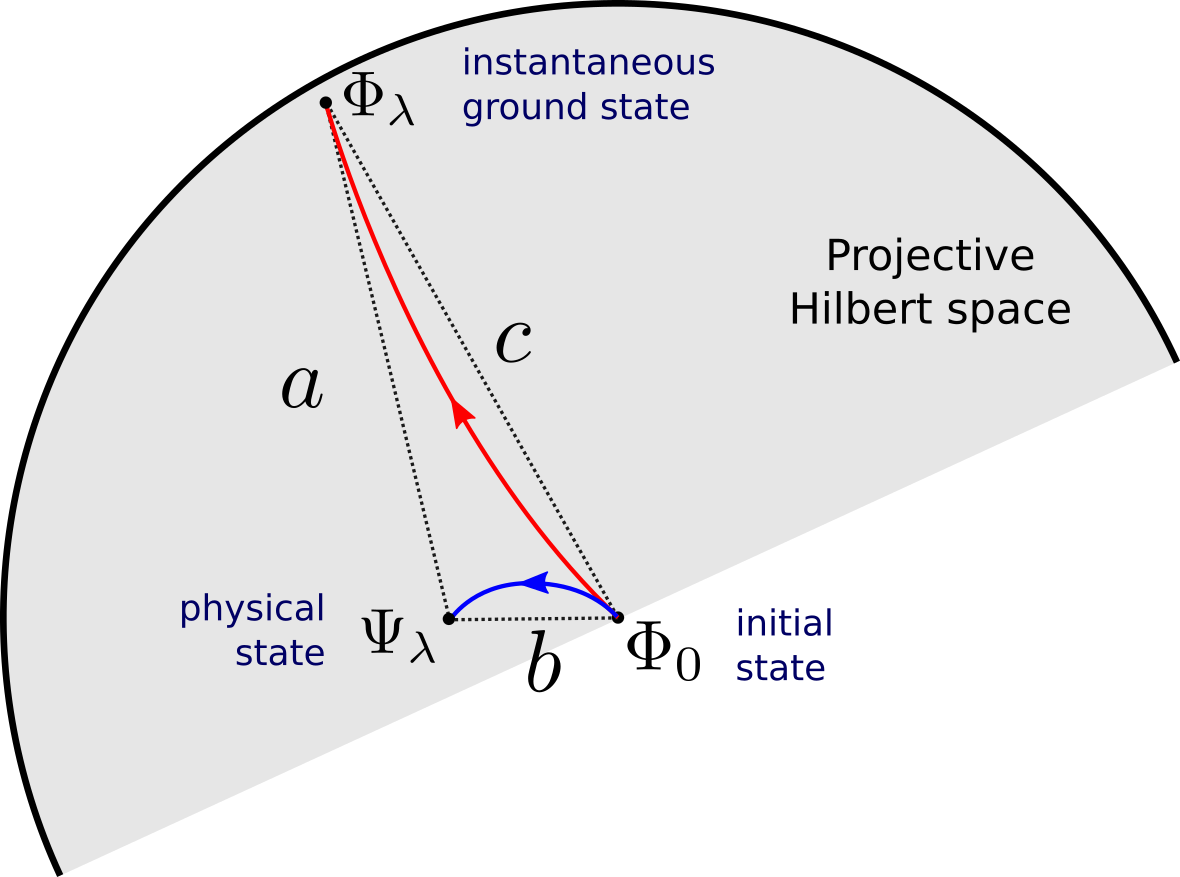
\includegraphics[width=1 \linewidth]{Fig_1.png}
%
\captionof{figure}{Triangle inequality resulting in the estimate Eq.~\eqref{inequality}. States are shown as
 points in the projective Hilbert space. The red trajectory shows the evolution of the
 instantaneous ground state, Eq.~\eqref{eigenproblem}, while the blue trajectory corresponds to the physical
 evolution given in  Eq.~\eqref{Schrodinger equation}. The length of the side $b$ is bounded by
 the quantum speed limit, while the length of the side $c$ approaches the
 maximally possible distance of $1$ in the large $N$ limit. \label{fig}}
\end{multicols}
\end{center}

\end{multicols}


\vspace{0.5 em}
%\vspace{3em} % When there are two boxes, some whitespace may need to be added if the one on the right has more content
}

%----------------------------------------------------------------------------------------
%
%----------------------------------------------------------------------------------------

\headerbox{4444 Adiabaticity breakdown time -- addressing \textbf{\textcolor{red}{Q1}}}{name=mfp,column=0,span=2,below=oc}{

\begin{multicols}{2}

Define the adiabaticity breakdown time $t_*$ and parameter $\lambda_*\equiv\lambda(t_*)$:
\begin{equation}\nonumber
\mathcal F(\lambda_*) =\frac{1}{e}.
\end{equation}
According to \eqref{inequality} and \eqref{CNdef},
\be\label{abt}\nonumber
\boxed{
\lambda_*=1/\sqrt{C_N}
}
\ee
up to small corrections as long as ${\cal R}(C_N^{-1/2})\ll 1$. The latter is guaranteed for sufficiently large system since
\be\label{1}\nonumber
\frac{\delta V_N}{C_N}\rightarrow0~~~{\rm for}~~~N \rightarrow \infty.
\ee
%{\small (proved for noninteracting fermions in a time-dependent potential; verified for other models).}
\vspace{0.2 em}








\end{multicols}
\vspace{0.2 em}
}




\headerbox{5555 Necessary condition for adiabaticity (\textbf{\textcolor{red}{Q2}})}{name=necessary,column=2,span=1,below=oc}{

If the orthogonality catastrophe is present, the adiabaticity can be maintained for finite systems only as long as ${\cal R}(\lambda_*)$ is large enough to make inequality \eqref{inequality} trivial. This entails
a \textbf{\textit{necessary adiabatic condition}:}
\be\nonumber
\Gamma_N <  \frac{\delta V_N}{2 C_N}\frac{1}{1-e^{-1}-\varepsilon}.
\ee
\vspace{0.7 em}
}

%%%%%%%%%%%%%%%%%%%%%%%%%%%%%%%%%%%%%%%%%%%%%%%%%%%%%%%%%%%%%%%%%%%%%%%%%%%%%%%%%%%%%%%%%%

\headerbox{6666 Quantized transport in Thouless pump}{name=expcons,column=0,below=mfp}{

%{\Large Thouless pump - a device which is able to transfer

\begin{center}
\begin{multicols}{2}
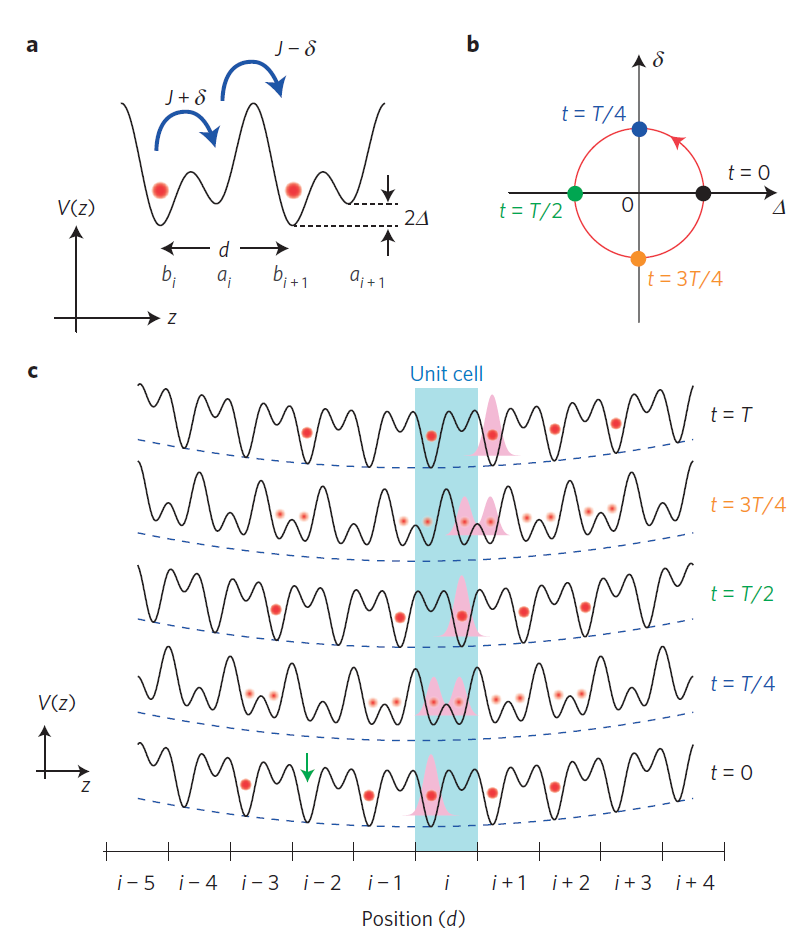
\includegraphics[width=0.9\linewidth]{fig_from_Nakajima.png}
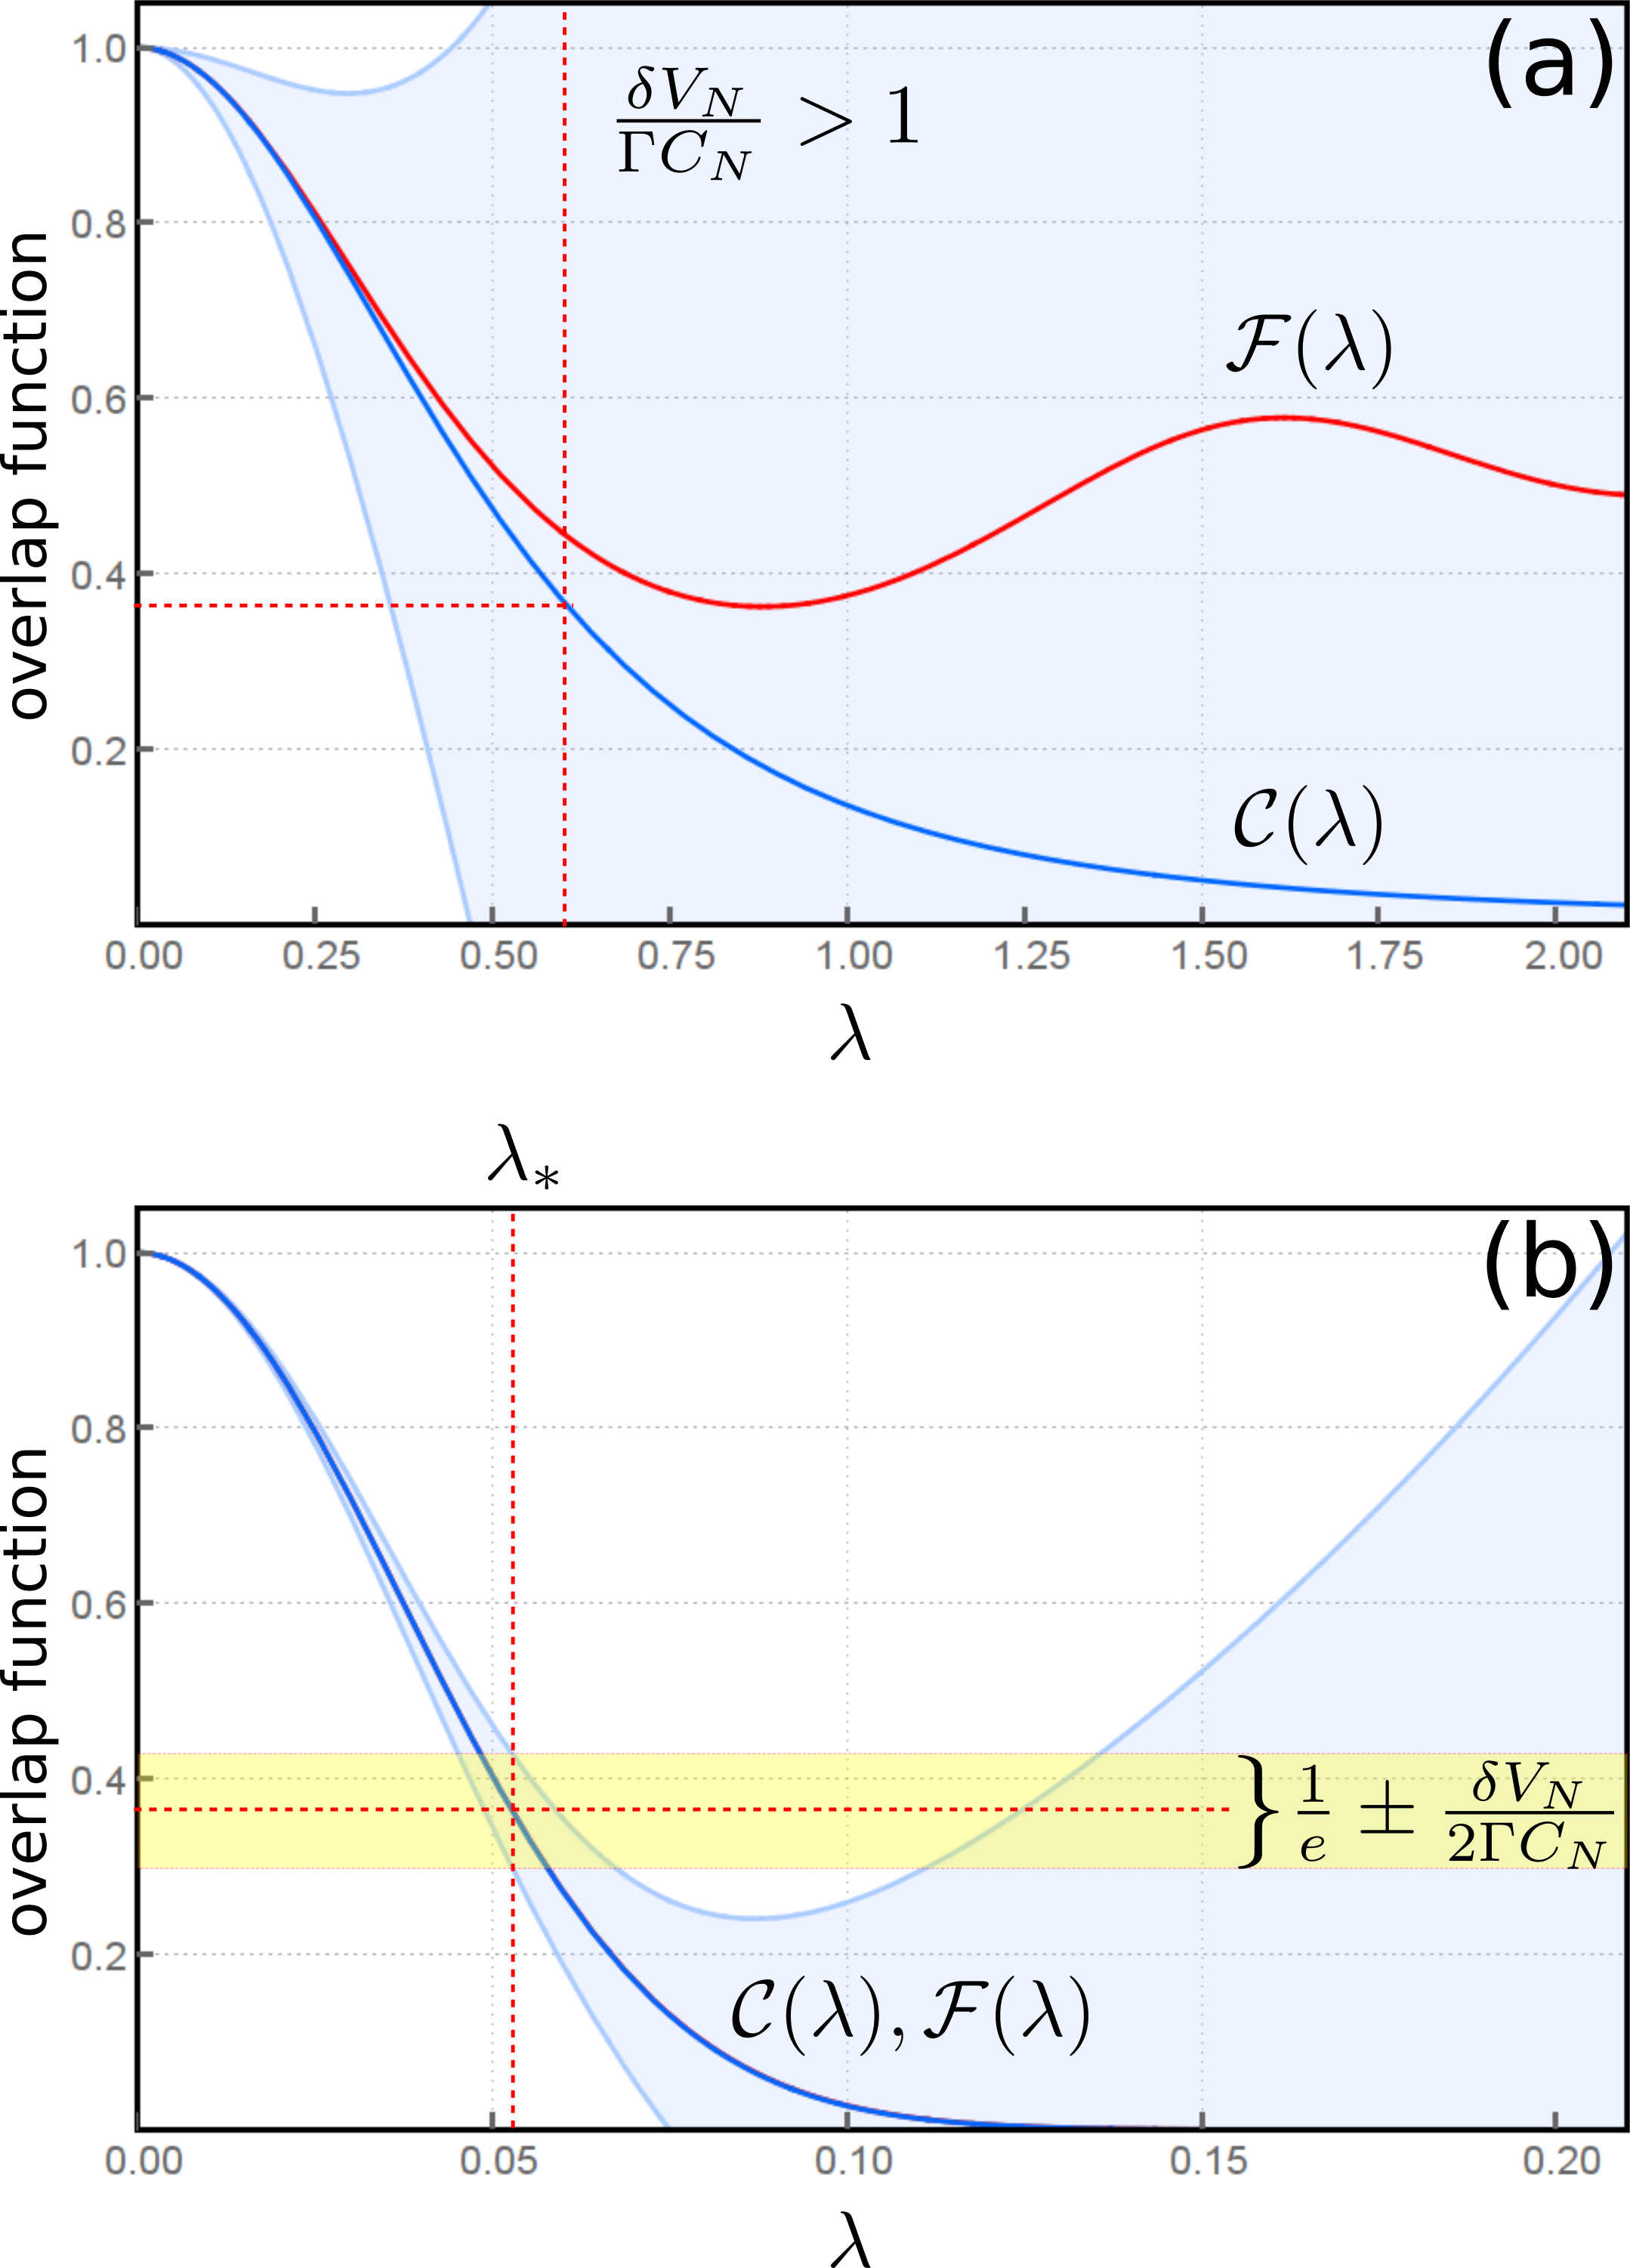
\includegraphics[width= 0.9 \linewidth]{Fig_2.png}
\end{multicols}

\captionof{figure}{Left: Thouless pump, figure from Ref. \cite{nakajima2016topological}. The pump transfers exactly one particle per cycle from left to right despite the fact that the coordinates of local minima of the potential remain constant. Right - evolution of the ground state fidelity in the parameter space
of the Hamiltonian \eqref{R-M} for (a) $N=10$, and (b) $N=1000$ particles.
%In panel (a) the fidelity $\mathcal F$ is shown as a solid red curve, while the overlap function $\mathcal C$ is shown as a solid blue curve.
The shaded region is the one, which has to contain the
$\mathcal F(\lambda)$ curve due to the inequality \eqref{inequality}.
For $N=10$ the inequality \eqref{inequality} does not impose a meaningful upper bound on the fidelity, and therefore
has nothing to say about the relationship between the fidelity and the orthogonality catastrophe.
In contrast, in panel (b) ($N=1000$) the bounds imposed by the inequality \eqref{inequality} are tight
enough, moreover, the two curves, $\mathcal C(\lambda)$ and
$\mathcal F(\lambda)$ are so close that look indistinguishable.
%The driving rate roughly corresponds to the pumping cycle period of $7$ ms.
\label{Thouless}
}
\end{center}

\vspace{2em}

Rice-Mele model: $N$ fermions in a time-dependent tight-binding lattice:
\begin{equation}
 H_{\rm RM}=
 \sum_{j=1}^N \left[-(J + \delta) a_j^\dagger b_j
 - (J - \delta) a_j^\dagger b_{j+1} + \mathrm {h.c.} \right]
 + \sum_{j=1}^N \Delta (a^\dagger_j a_j - b^\dagger_j b_j ) .
 \label{R-M}
\end{equation}

\be\nonumber
\Delta(\lambda)=\Delta_{\rm max}\cos\lambda,~~~\delta(\lambda)=\delta_{\rm max}\sin\lambda
\ee

At the point $\lambda=\pi/4$
\begin{equation}\label{CN R-M spec}\nonumber
C_N=\frac{N \Delta^2}{16 J \delta},~~~~ \delta V_N^{\rm RM}=\sqrt N \Delta.
\end{equation}

\begin{multicols}{2}

Adiabaticity breakdown time:

$$
\boxed{
t_*=\frac{1}{\Gamma \sqrt{N} }\frac{4\sqrt{J \delta}}{\Delta}
}
$$
\newpage
Necessary adiabatic condition:
$$
\boxed{
\Gamma_N<\frac{1}{\sqrt{N} }\frac{16J \delta}{\Delta}
}
$$

\end{multicols}


\vspace{0.1 em}

}

%%%%%%%%%%%%%%%%%%%%%%%%%%%%%%%%%%%%%%%%%%%%%%%%%%%%%%%%%%%%%%%%%%%%%%%%%%%%

\headerbox{777 Two modes of operation of  Thouless pump}{name=regimes,column=1,below=mfp}{

 Quantum many-body adiabaticity in a strict sense \eqref{adiabaticity} is implied in the original derivation by Thouless \cite{thouless1983quantization}. But is it is really necessary for quantization of transport? Yes and No. This depends on the mode of operation of the Thouless pump.

\begin{itemize}
  \item Mode 1: A single cycle is performed, the transferred charge is measured immediately after the cycle is over. Many-body quantum adiabaticity is {\it not required}.
  \item Mode 2: Pump is operated continuously (one cycle after another) in a stationary state, charge transferred per cycle is measured. Many-body quantum adiabaticity is {\it indispensable}.
  \item Mode 2': A single cycle is performed, but the transferred charge is measured after large time after the cycle is over. Many-body quantum adiabaticity is {\it indispensable}.
\end{itemize}


\begin{center}
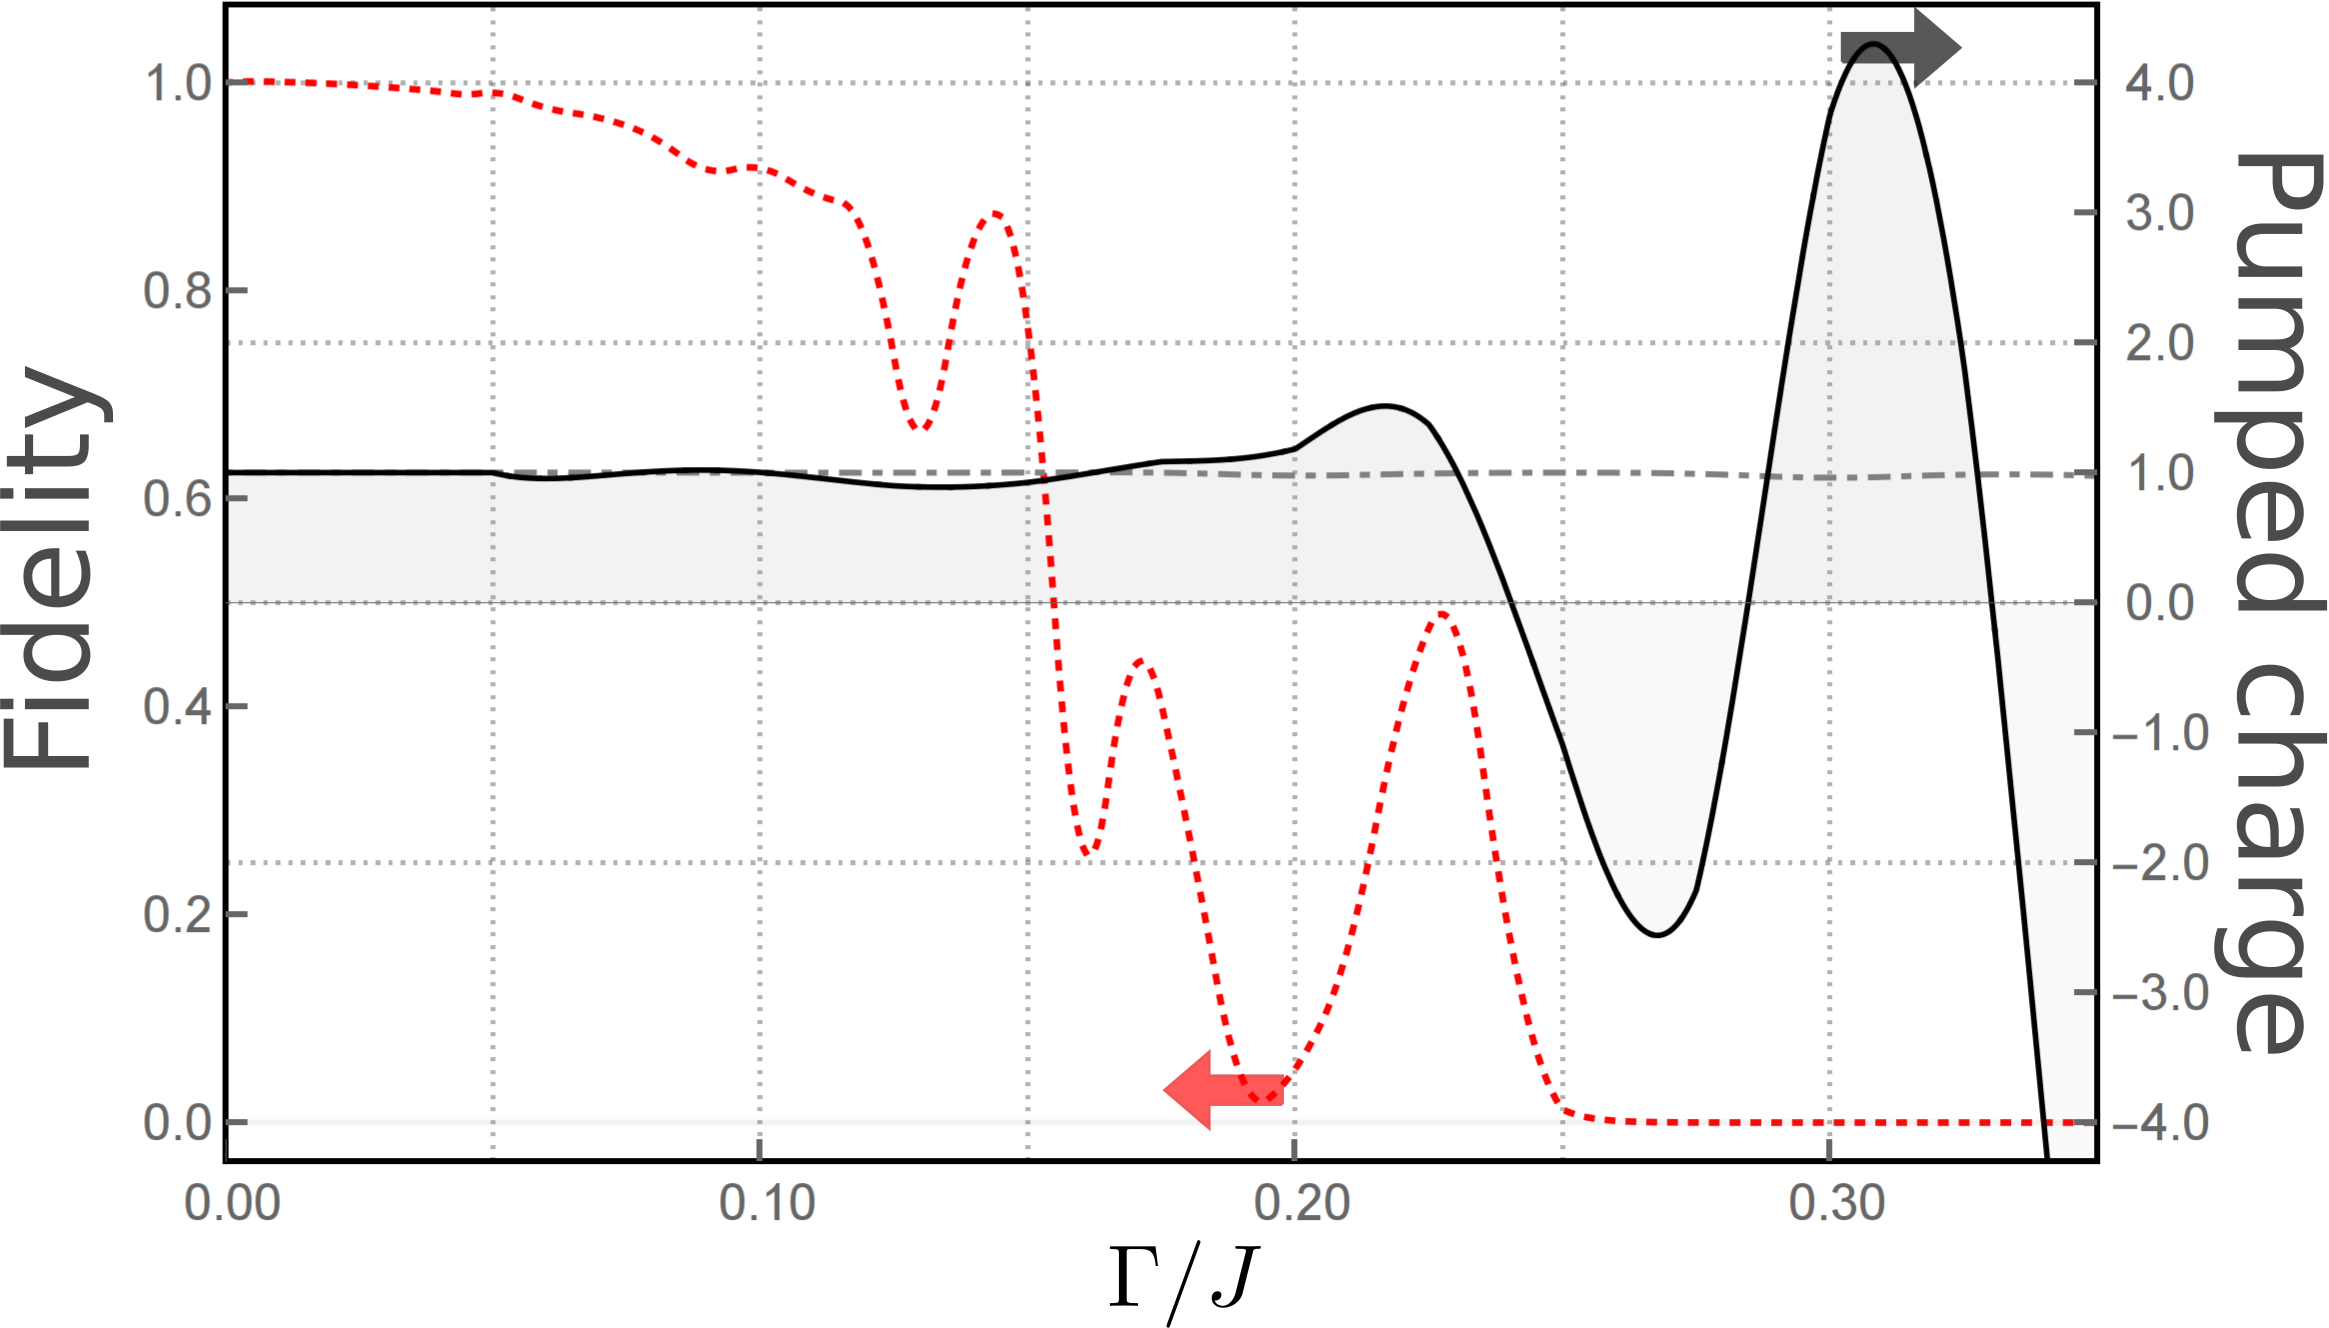
\includegraphics[width=0.8\linewidth]{Fig_4_v2.png}
\captionof{figure}{
Operation of the Rice-Mele realization of the Thouless pump, eq. \eqref{R-M}, in the first cycle as compared
to a steady-state regime. Calculations are done
for $N=1000$ and different values of the driving rate, $\Gamma$. The cycle is given by $\Delta=(J/2)\sin\lambda$, $\delta=(J/2)\cos\lambda$ with
$\lambda=\Gamma t$. Initially the system is in equilibrium. Dash-dotted gray -- charge transferred in the first cycle. Dashed red -- the adiabatic fidelity
$\mathcal F$ at the end of the first cycle. Solid black --
charge transferred per cycle in a continuous regime after the stationary state is reached.  One can see that the charge transferred in the first cycle is quantized even when the
many-body adiabaticity has gone completely ($\mathcal F\simeq0$), while the quantization of the charge in the continuous regime
disappears as soon as the many-body adiabaticity is broken.   \label{fig 4}}
\end{center}

\vspace{0.5 em}

 Qualitative reason:
When the adiabaticity is broken,  $\delta N \sim \sqrt N$ elementary excitations are produced during one cycle.
\begin{itemize}
  \item Mode 1: Only $ (v T/a) \delta N/N\sim 1/\sqrt N$ of these excitations leave the pump through its end points during the first cycle. Here $v$ is the average velocity of excitations. Their effect is {\it negligible} in the thermodynamic limit.
  \item Mode 2: In a stationary state number of excitations which leave the pump per cycle is equal to the number of excitations created per cycle due to driving, $\delta N \sim \sqrt N$. Their effect {\it diverges} in the thermodynamic limit.
\end{itemize}




}

%%%%%%%%%%%%%%%%%%%%%%%%%%%%%%%%%%%%%%%%%%%%%%%%%%%%%%%%%%%%%%%%%%%%%%%%%%%%

\headerbox{8888 Simple but important corollary}{name=corollary,column=2,span=1,below=mfp}{

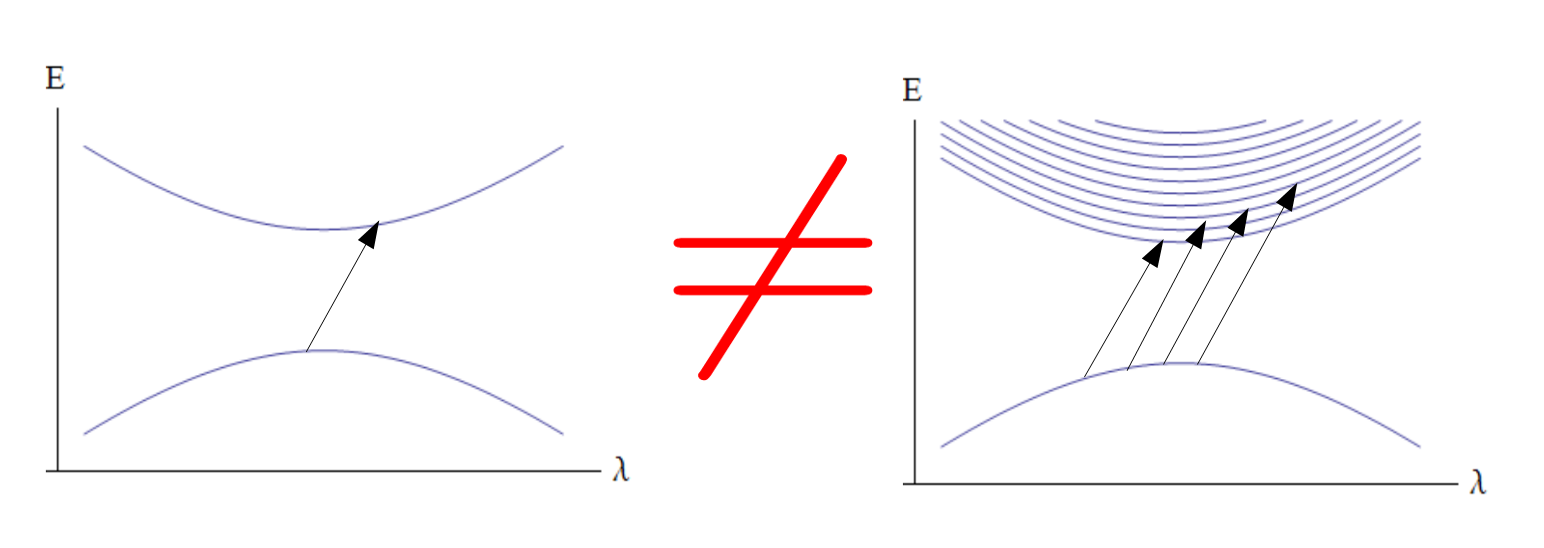
\includegraphics[width=0.9\linewidth]{2level-mb.png}

\begin{multicols}{2}

In a two-level system adiabaticity is governed by the gap ( Landau-Zener). Adiabatic condition reads
$$
\Gamma\ll\Delta E_{\rm min}.
$$

\newpage

A Landau-Zener-type guess is typically \textcolor{red}{\textbf{completely wrong}} for bulk driven many-body systems!
For a gapped system the adiabatic condition reads
$$
\Gamma\ll f_N\,\, \Delta  E_{\rm min}~~~ {\rm with} ~~~ \lim_{N\rightarrow\infty}f_N=0.
$$

\end{multicols}


\vspace{0.3 em}
}

\vspace{0.5 em}

\headerbox{999 Summary and concluding remarks}{name=summary,column=2,span=1,below=corollary}{
{\large


\begin{itemize}
\item Adiabaticity breakdown in many-body systems is closely related to the orthogonality catastrophe.
\item The adiabaticity breakdown time $t_*$ vanishes in the thermodynamic limit.
\item Scaling of $t_*$ with the number of particles, $N$, is determined by the nature of driving (global or local) and by presense/absense of gapless excitations.
\item Contrary to the common belief, whenever driving is of bulk type, \textcolor{red}{even a finite gap is not able to protect adiabaticity in the thermodynamic limit!}
\item Necessary adiabatic condition for finite systems derived -- the most stringent to date, to the best of our knowledge!
\item Quantum many-body adiabaticity is mandatory for the quantized particle transport in a topological Thouless pump operated continuously. However, adiabaticity breakdown does not spoil quantization in the first few cycles, if initially the pump is in the ground state. In other words,  the quantization of the transport under nonadiabatic conditions is necessarily a transient phenomenon.
\end{itemize}
}

\vspace{1 em}

}


%----------------------------------------------------------------------------------------
%	LITERATURE
%----------------------------------------------------------------------------------------

\headerbox{References}{name=references,column=0,below=regimes,span=3}{
{\small
\begin{multicols}{3}

\renewcommand{\section}[2]{\vskip 0.05em} % Get rid of the default "References" section title
%\nocite{*} % Insert publications even if they are not cited in the poster
%\small{ % Reduce the font size in this block
\bibliographystyle{abbrv}
%unsrt
%
%\bibliography{C:/D/Work/QM/Bibs/1D,C:/D/Work/QM/Bibs/He} % Use sample.bib as the bibliography file
\bibliography{D:/Work/QM/Bibs/1D,D:/Work/QM/Bibs/LZ_and_adiabaticity,D:/Work/QM/Bibs/orthogonality_catastrophe}
%}
\end{multicols}
}
}

\end{poster}

\end{document}

